\documentclass{minimal}

\usepackage{tikz}
\usepackage{amsmath}
\usepackage{amssymb}
\usepackage{amsfonts}

\begin{document}

\pagestyle{empty}

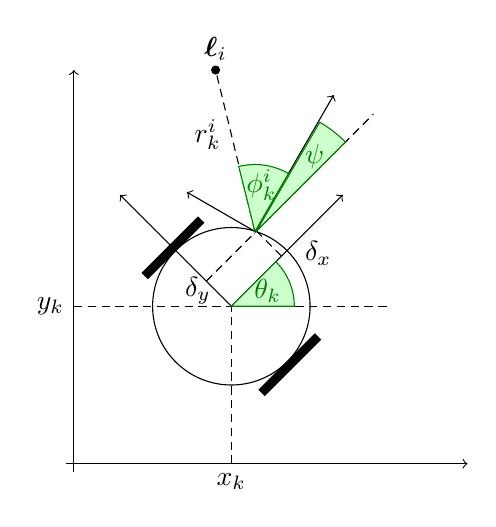
\begin{tikzpicture}[]
  % styles
  \tikzstyle{axes}=[]
  \tikzstyle{robot} = []
  \tikzstyle{wheels} = [fill]
  \tikzstyle{landmark} = [fill]
  \tikzstyle{lrf measurement} = [densely dashed]
  \colorlet{anglecolor}{green!50!black}

  % world axes
  \begin{scope}[style = axes]
    \draw[->] (-0.1, 0) -- (5, 0);
    \draw[->] (0, -0.1) -- (0, 5);
  \end{scope}

  % robot base
  \begin{scope}[style = robot, xshift = 2cm, yshift = 2cm, rotate = 45]
    \draw (0, 0) circle (1);
    \draw[wheels] (-0.5, 1) rectangle (0.5, 1.1);
    \draw[wheels] (-0.5, -1) rectangle (0.5, -1.1);
  \end{scope}

  % robot axes
  \begin{scope}[style = axes, xshift = 2cm, yshift = 2cm, rotate = 45]
    \draw[->] (0, 0) -- (2, 0);
    \draw[->] (0, 0) -- (0, 2);
  \end{scope}

  % lrf axes
  \begin{scope}[style = axes, xshift = 2.3cm, yshift = 2.95cm, rotate = 60]
    \draw[->] (0, 0) -- (2, 0);
    \draw[->] (0, 0) -- (0, 1);
  \end{scope}

  % landmark
  \begin{scope}[style = landmark, xshift = 1.8cm, yshift = 5cm, rotate = 0]
    \draw[landmark] (0, 0) circle (0.05) node[above] {$\boldsymbol{\ell}_i$};
  \end{scope}

  % lrf range measurement
  \begin{scope}[style = lrf measurement]
    \draw (2.3, 2.95) -- (1.8, 5) node[left = 0.1cm, below = 0.5cm] {$r^i_k$};
  \end{scope}

  % lrf bearing measurement
  \begin{scope}[xshift = 2.3cm, yshift = 2.95cm, rotate = 60]
    \filldraw[fill = green!20, draw = anglecolor] (0, 0) -- (8.5mm, 0) arc
      (0:44:8.5mm) -- cycle;
    \draw (22:6mm) node[anglecolor] {$\phi^i_k$};
  \end{scope}

  % robot pose
  \begin{scope}
    \draw[densely dashed] (2, 0) node[below] {$x_k$} -- (2, 2);
    \draw[densely dashed] (0, 2) node[left] {$y_k$} -- (4, 2);
    \filldraw[fill = green!20, draw = anglecolor] (2, 2) -- (2.8, 2) arc
      (0:45:0.8) -- cycle;
    \draw[xshift = 2cm, yshift = 2cm] (22.5:0.5) node[anglecolor] {$\theta_k$};
  \end{scope}

  % lrf pose
  \begin{scope} [xshift = 2cm, yshift = 2cm, rotate = 45]
    \draw[densely dashed] (0.9, 0) node[below = -1pt, right = 5pt] {$\delta_x$} -- (0.9, 0.45);
    \draw[densely dashed] (0, 0.45) node[left = 3pt, below = -5pt] {$\delta_y$} -- (3, 0.45);
    \filldraw[fill = green!20, draw = anglecolor] (0.9, 0.45) -- (2.5, 0.45) arc
      (0:14.8:1.6) -- cycle;
    \draw[xshift = 0.9cm, yshift = 0.45cm] (7:1.2) node[anglecolor] {$\psi$};
  \end{scope}

\end{tikzpicture}
\end{document}
